\documentclass[tikz,border=8pt]{standalone}
% Shared look for every TikZ diagram. Load with \input{../../tools/tikz-style.tex}
\usepackage[T1]{fontenc}
\usepackage{lmodern}
\renewcommand{\sfdefault}{lmr}  % diagrams use the same serif as the text
\usetikzlibrary{arrows.meta, positioning, shapes.geometric, calc, fit, backgrounds}
\definecolor{cblue}{HTML}{4C78A8}
\definecolor{corange}{HTML}{F58518}
\definecolor{cgreen}{HTML}{54A24B}
\definecolor{cred}{HTML}{E45756}
\definecolor{cpurple}{HTML}{B279A2}
\definecolor{cgrey}{HTML}{6B6B6B}
\tikzset{
  every picture/.style={font=\sffamily, line width=1.2pt},
  box/.style={draw=#1, fill=#1!12, rounded corners=4pt, align=center, inner sep=7pt, minimum height=1.1cm},
  box/.default=cgrey,
  arrow/.style={-{Stealth[length=3mm]}, draw=cgrey, line width=1.4pt},
  title/.style={font=\sffamily\bfseries\Large},
  note/.style={font=\sffamily\small, text=cgrey, align=center},
}
\AtBeginDocument{\hyphenpenalty=10000 \exhyphenpenalty=10000}

\begin{document}
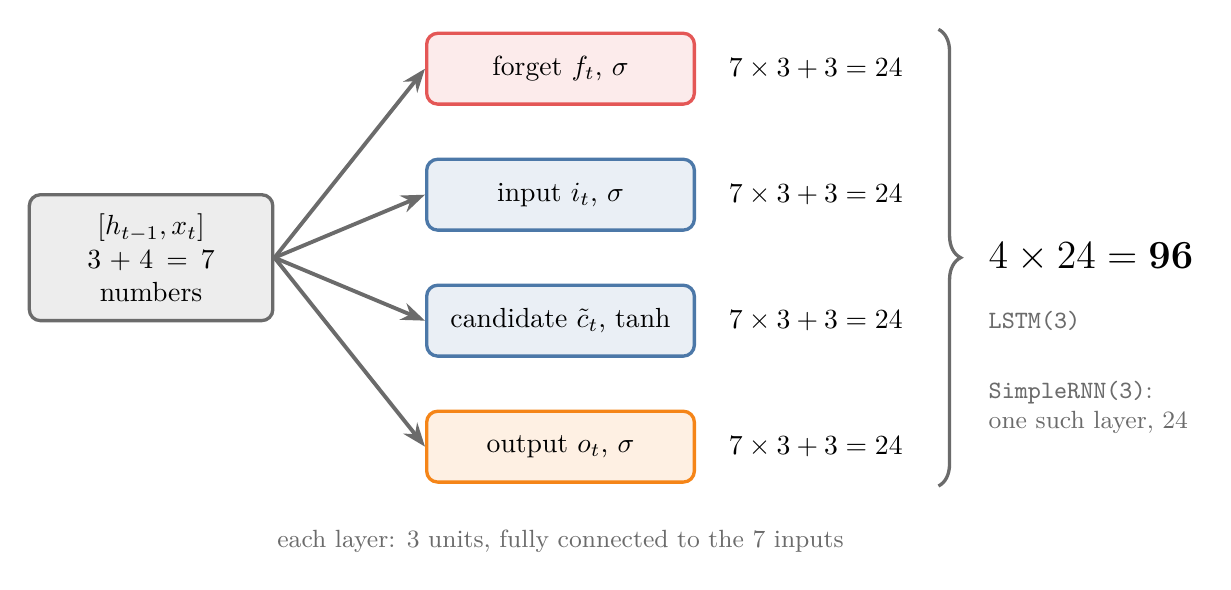
\begin{tikzpicture}[lay/.style={box=#1, minimum width=3.4cm, minimum height=0.9cm, font=\sffamily}]
  \node[box=cgrey, text width=2.6cm] (in) at (0,0) {$[h_{t-1}, x_t]$\\ $3 + 4 = 7$ numbers};
  \foreach \n/\col/\lab/\y in {f/cred/{forget $f_t$, $\sigma$}/2.4, i/cblue/{input $i_t$, $\sigma$}/0.8, c/cblue/{candidate $\tilde c_t$, tanh}/-0.8, o/corange/{output $o_t$, $\sigma$}/-2.4} {
    \node[lay=\col] (\n) at (5.2,\y) {\lab};
    \draw[arrow] (in.east) -- (\n.west);
    \node[anchor=west, font=\sffamily] at (7.2,\y) {$7 \times 3 + 3 = 24$};
  }
  \draw[decorate, decoration={brace, amplitude=8pt}, cgrey] (10.0,2.9) -- (10.0,-2.9);
  \node[anchor=west, font=\sffamily\Large] at (10.5,0) {$4 \times 24 = \mathbf{96}$};
  \node[note, anchor=west] at (10.5,-0.8) {\texttt{LSTM(3)}};
  \node[note, anchor=west, align=left] at (10.5,-1.9) {\texttt{SimpleRNN(3)}:\\one such layer, 24};
  \node[note] at (5.2,-3.6) {each layer: 3 units, fully connected to the 7 inputs};
\end{tikzpicture}
\end{document}
